\documentclass{beamer}
\usepackage[utf8]{inputenc}
\usepackage[spanish]{babel}
\usepackage{hyperref}
\usepackage{verbatim}
\usepackage{listings}
\usepackage{tikz}
\usepackage{ulem}
\usetikzlibrary{arrows}

\setbeamercovered{invisible}
\usetheme{Frankfurt}
\usefonttheme{serif}

% Configurar los listings (Códigos)
\renewcommand{\lstlistingname}{Código}
\lstset{
	language=C++,               % Lenguaje
	basicstyle=\ttfamily\tiny,  % Tipo de fuente
	keywordstyle=\color{blue},  % Color de palabras clave
	stringstyle=\color{red},    % Color de strings
	commentstyle=\color{gray},  % Color de comentarios
	showstringspaces=false,     % No muestrar el _ cuando el string tiene espacios
	breaklines = true,          % Partir las líneas largas
	breakatwhitespace=true,	    % Partir las líneas en un espacio
	numbers=left,				% Numerar las líneas a la izq
	numberstyle=\tiny,			% Poner los números de las líneas pequeños
	numberblanklines=true,      % Numerar las líneas en blanco
	columns=fullflexible,       % No perder el formato al dejar los espacios
	keepspaces=true,   			% Dejar los espacios insertados
	frame=tb,					% Poner el recuadro
}


\AtBeginSection[]{%
  \begin{frame}<beamer>
    \frametitle{Contenido}
    \tableofcontents[sectionstyle=show/hide,subsectionstyle=hide/show/hide]
  \end{frame}
  \addtocounter{framenumber}{-1}% If you don't want them to affect the slide number
}


\title{Desarrollo e implementación de un programa de trabajo para el semillero de programación}
\author{Por: \\ Ana Echavarría Uribe \\ \quad \\ Tutor: \\ Juan Francisco Cardona Mc'Cormick}

\institute{Universidad EAFIT}
\date{26 de abril de 2013}

\begin{document}

\begin{frame}
	\titlepage
\end{frame}

\begin{frame}
	\frametitle{Contenido}
	\tableofcontents
\end{frame}

\section[Informe anterior]{Resumen informe anterior}

	\begin{frame}
		\frametitle{Objetivo General}
		\begin{block}{}
			Desarrollar e implementar un plan de actividades y temas de fundamentación matemática para el semillero de programación que busque mejorar las habilidades de programación de los estudiantes, basándose en la metodología usada por Steven Halim en el curso Competitive Programming de la Universidad Nacional de Singapur y en otras que en el desarrollo del proyecto puedan surgir.
		\end{block}
	\end{frame}
	
	\begin{frame}
		\frametitle{En el informe anterior}
		\begin{itemize}
			\item Quién es Steven Halim y cuál es su metodología de trabajo para el curso competitive programming.
			\item Comparación entre la metodología de Steven Halim y la metodología con la que se está desarrollando el Semillero.
			\item Temas vistos en el Semillero hasta la fecha
		\end{itemize}
	\end{frame}

\section[Curso Stanford]{Curso ``Algorithms: Design and Analysis'' }

	\begin{frame}
		\frametitle{Algorithms: Design and Analysis Part 1 / Part 2}
		\begin{itemize}
			\item Dos cursos abiertos dictados por el profesor Tim Roughgarden de Stanford
			\item Duración: 6 semanas cada uno.
			\item La versión de este curso en Stanford está enfocada a estudiantes de 2do y 3er año de ciencias de la computación.
			\item La clase consiste en videos de 10 a 15 minutos de duración, exámenes y prácticas de programación.
		\end{itemize}	
	\end{frame}
	
	\begin{frame}
		\frametitle{Algorithms: Design and Analysis Part 1 / Part 2}
		\begin{itemize}
			\item Enseña los seudocódigos mas no las implementaciones en código.
			\item Cubre la mayoría de los algoritmos programados para ver en el semillero.
			\item Material abierto al público en \url{https://www.coursera.org/course/algo/} y \url{https://www.coursera.org/course/algo2}
		\end{itemize}	
	\end{frame}
	
	\begin{frame}
		\frametitle{Tim Roughgarden}
		\begin{center} 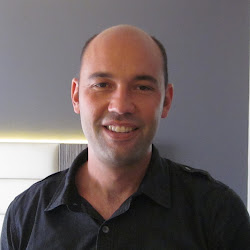
\includegraphics[height = 0.25\textheight]{Tim.jpg} \end{center}
		\begin{itemize}
			\item Profesor de ciencias de la computación de Stanford.
			\item Profesor de diseño y análisis de algoritmos desde hace 8 años.
			\item Investigador en teoría y aplicaciones de algoritmos.
			\item Profesor de los cursos abiertos de ``Algorithms: Design and Analysis Part 1 / Part 2''. 
		\end{itemize}
	\end{frame}
	


\section[Curso MIT]{Curso ``Introduction to Algorithms''}
	\begin{frame}
		\frametitle{Introduction to Algorithms}
		\begin{itemize}
			\item Parte del contenido de los cursos abiertos de MIT.
			\item Cubre temas como estructuras de datos, programación dinámica, algoritmos de grafos, entre otros.
			\item Dictado por los profesores Charles Leiserson y Erik Demaine.
		\end{itemize}
	\end{frame}
	
	\begin{frame}
		\frametitle{Introduction to Algorithms}
		\begin{itemize}
			\item Tiene como prerrequisitos buenas bases de programación, matemáticas discretas y probabilidad.
			\item Enseña los seudocódigos mas no las implementaciones en código.
			\item Material abierto al público en \url{http://ocw.mit.edu/courses/electrical-engineering-and-computer-science/6-046j-introduction-to-algorithms-sma-5503-fall-2005/}
		\end{itemize}
	\end{frame}
	
	\begin{frame}
		\frametitle{Charles Leiserson y Erik Demaine}
		\begin{columns}[l]
			\column{0.45\textwidth}
				\begin{center} 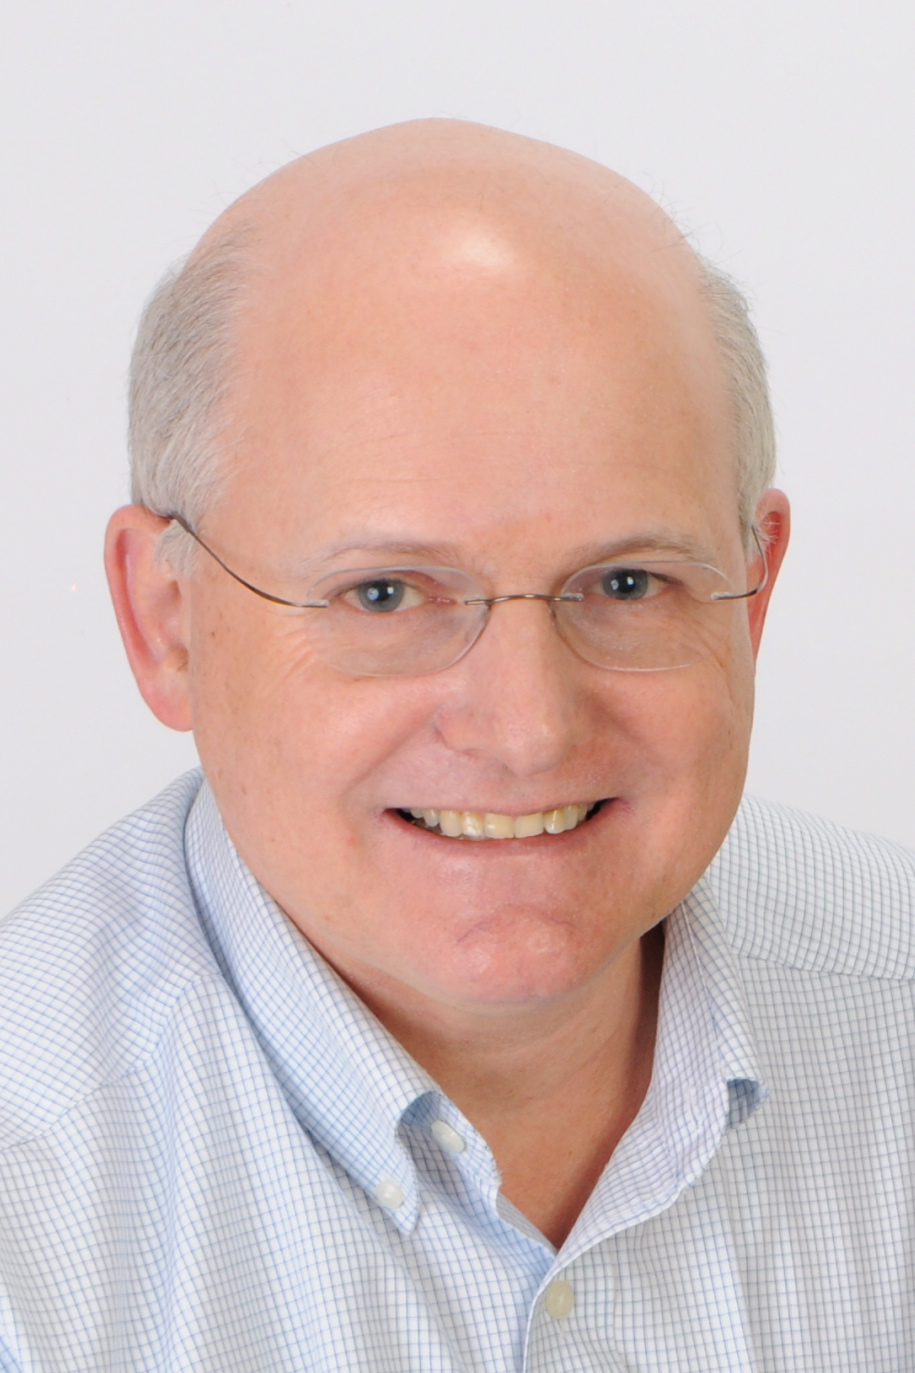
\includegraphics[height = 0.25\textheight]{Leiserson.jpg} \end{center}
				\begin{itemize}
					\item Profesor de ciencias de la computación e ingeniería de MIT.
					\item Co-autor del libro ``Introduction to Algorithms''.
				\end{itemize}
			\column{0.45\textwidth}
				\begin{center} 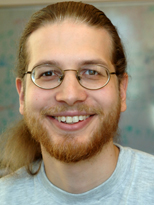
\includegraphics[height = 0.25\textheight]{Demaine.jpg} \end{center}
				\begin{itemize}
					\item Profesor de ciencias de la computación de MIT.
					\item Investigación en algoritmos, estructuras de datos y teoría de juegos.
				\end{itemize}
		\end{columns}
	\end{frame}
	
\section[Temas vistos]{Temas vistos en el Semillero de Programación}
	\begin{frame}
		\frametitle{Temas vistos}
		\begin{enumerate}
			\item{Algoritmo de Bellman-Ford}
			\item{Programación dinámica}
			\item{Algoritmo de Floyd-Warshall}
			\item{Árbol de mínima expansión}
			\item{Algoritmo de Knuth-Morris-Pratt}
		\end{enumerate}
	\end{frame}
	
	\begin{frame}
		\frametitle{Competencias}
		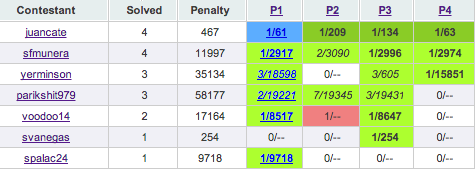
\includegraphics[width = \textwidth]{Contest1.png}\\ \quad \\
		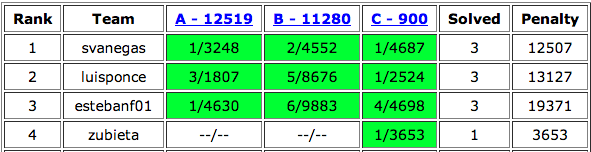
\includegraphics[width = \textwidth]{Contest2.png}
	\end{frame}
	

\section[Contenido en Github]{Contenido del Semillero en Github}
	\begin{frame}
		\frametitle{Contenido del Semillero en Github}
		\begin{itemize}	
			\item El contenido del Semillero se almacena en un repositorio en \url{https://github.com/anaechavarria/SemilleroProgramacion}
			\item Se decidió compartir el contenido del repositorio con el coach de maratones de la Universidad Tecnológica de Pereira.
			\item El coach difundió la información entre sus estudiantes.
		\end{itemize}
	\end{frame}
	
	\begin{frame}
		\frametitle{Contenido del semillero en Github}
		\begin{itemize}
			\item 8 personas nuevas empezaron a seguir mi contenido y otras 3 personas marcaron el repositorio como favorito.
			\item Un estudiante de la Universidad Sergio Arboleda pidió permiso para usar el contenido como material de aprendizaje para él y su equipo.
			\item Se está mirando para compartir el contenido con estudiantes de la Universidad Pontificia Bolivariana.
		\end{itemize}
	\end{frame}
	
	\begin{frame}
		\frametitle{Contenido del semillero en Github}
		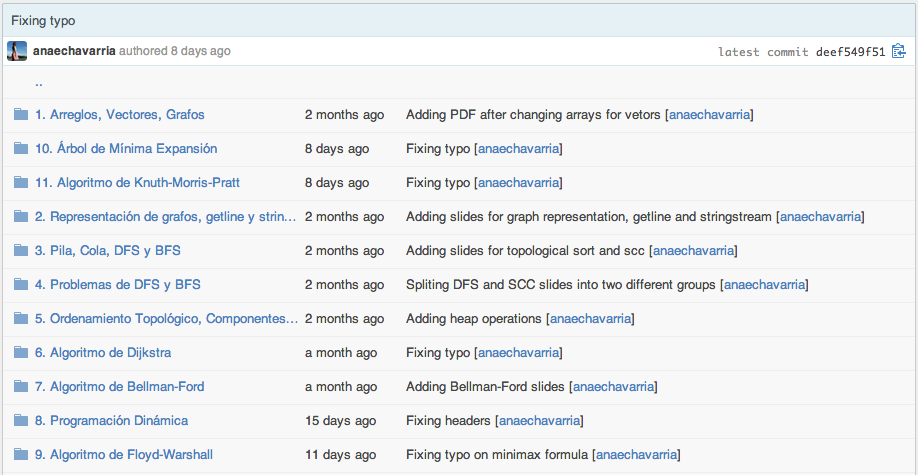
\includegraphics[width = \textwidth]{Repo.png}
	\end{frame}
	
\section[Preguntas]{Preguntas}
	\begin{frame}
		\frametitle{Preguntas}
		
\includegraphics[width = 0.9\textwidth]{preguntas.jpeg}
	\end{frame}

\end{document}